\documentclass[a4paper,12pt]{article}
\usepackage{relsize}
\usepackage[margin=3cm]{geometry} %Definiere Rand
\usepackage{graphicx} % Zum Einbinden von Bildern
\usepackage[english]{babel} % Direkte Eingabe von Umlauten
\usepackage[utf8]{inputenc} % Direkte Eingabe von Umlauten
\usepackage[T1]{fontenc}  % Direkte Eingabe von Umlauten
\usepackage{pgfplots} % Zum Einfuegen von Plots
\pgfplotsset{compat=1.14} % Damit wird beim Plotten keinen Error bekommen
\usepackage[section]{placeins} %Damit Bilder in der Section bleiben
\usepackage{amsmath} % Standard fuer mathematische Ausdruecke
\usepackage{amssymb} % Weitere Symbole
\usepackage{mathtools} % Fuer weitere mathematische Ausdruecke
\usepackage{siunitx} % Um SI-Einheiten anzugeben
\usepackage[font=small,labelfont=bf]{caption} % Kleinerer Text bei Captions
\usepackage{tabu} % Anderes Tabellenenvironment, wird am Ende fuer die Namen verwendet
\usepackage{subcaption} % Side-by-side figures with minipage
\usepackage{url} % Damit man urls zitieren kann
\usepackage[autostyle=true,german=quotes]{csquotes} % Damit Zitieren leichter ist; Bsp: \enquote{nur}
\usepackage[nottoc,numbib]{tocbibind} % Damit die Referenzen im Inhaltsverzeichnis erscheinen
% Die folgenden zwei Zeilen benennen "Inhaltsverzeichnis" zu "Referenzen um
\usepackage{standalone} % Zum Outsourcen von Plots
\addto\captionsngerman{\renewcommand{\bibname}{Referenzen} \renewcommand{\refname}{Referenzen}} % Benennt "Literatur" in "Referenzen" um
\sisetup{range-phrase=-} % Wie SI-Intervalle angezeigt werden
\usepackage{setspace} % Damit die naechsten funktionieren
\renewcommand{\topfraction}{0.85} % Let top 85% of a page contain a figure
\renewcommand{\textfraction}{0.1} % Default amount of minimum text on page (Set to 10%)
\renewcommand{\floatpagefraction}{0.75} % Only place figures by themselves if they take up more than 75% of the page
\DeclareSIPostPower\tothefourth{4} % SI-Einheiten zur 4. Potenz
%
\makeatletter
\newcommand*{\rom}[1]{\expandafter\@slowromancap\romannumeral #1@}
\makeatother %roman numerals
\usepackage{threeparttable, tablefootnote}
\DeclareSIUnit\torr{torr}
\usepackage{circuitikz} %For circuits
\renewcommand{\d}{\mathrm{d}}
\newcommand{\intl}{\int\limits}
\sisetup{math-micro=\text{µ},text-micro=µ}
\usepackage{hyperref} % For hyperlinks to be clickable
\begin{document}
%
    \title{[Title of thesis]\\
    \vspace{2em}
    Bachelorarbeit\\
    \vspace{2em}
    \smaller[2]{}zur Erlangung des akademischen Grades\\
    Bachelor of Science (BSc)\\
    \vspace{2em}
    eingereicht an der\\
    Fakult{\"a}t f{\"u}r Mathematik, Informatik und Physik\\
    der\\
    Leopold-Franzens-Universit{\"a}t Innsbruck\\
    \vspace{1.5em}
    von}

    \author{
 	\LARGE Bernhard Gstrein\\
 	\vspace{.5em} \\
 	Betreuer:\\
 	Univ.Prof. Dr. Helmut Ritsch\\
 	\small Institut f{\"u}r Theoretische Physik\\
 	\vspace{1em}
	}
    
    \date{Innsbruck, 2019}

    \maketitle
   
   \begin{abstract}
	Hier die Kurzfassung in ganzen Sätzen.
	\end{abstract}
   
\newpage
   
\tableofcontents
 
\newpage
    

\section{Pumped cavity}
The derivation for the Hamiltonians for the following sections is taken from \cite{donner}.

\subsection{Longitudinal Pump}
In the simulation we set the external Potential to 0. We set $U_0 \coloneqq g_0^2/\Delta a$. Since we are working with a red-detuned laser, $\Delta a$ and $\Delta c$ are smaller 0. The Hamiltonian is:

\begin{align}
H_\text{long} = \frac{p^2}{2m} + V_\text{ext}(x) - \hbar \Delta_c a^\dagger a + \hbar \eta (a + a^\dagger) + \hbar U_0 \cos(kx)^2 a^\dagger a.
\end{align}We want to make sure all quantities are expressed with the recoil energy $E_r = \hbar \omega_r$, where $\omega_r = \hbar k^2 / 2m$ is the recoil frequency. Therefore we factor our $E_r$ to see what we have to type into the program:

\begin{align}
\begin{split}
H_\text{long} = \hbar \omega_r \biggl( \frac{1}{\hbar^2 k^2} p^2 + \frac{1}{\hbar \omega_r} V_\text{ext}(x) - \frac{1}{\omega_r} \Delta_c a^\dagger a + \frac{1}{\omega_r} \eta (a + a^\dagger) + \\
 + \frac{1}{\hbar \omega_r} U_0 \cos(kx)^2 a^\dagger a \biggr).
\end{split}
\end{align}In the simulation program, we will thus set $\hbar = 1$ and divide each quantity by the preceding factors.

\subsection{Transversal pump}
Again, in the simulation we set the external potential to 0. Here we only consider one dimension, so we set $z=0$.

\begin{align}
\begin{split}
H_\text{transv} = \frac{p^2}{2m} + V_\text{ext}(x) - \hbar \Delta_c a^\dagger a - \hbar \eta \cos(kx) \cos(kz) (a + a^\dagger) + \\
 + \hbar U_0 \cos(kz)^2 + \hbar U_0 \cos(kz)^2 a^\dagger a.
\end{split}
\end{align}As previously mentioned, keeping the right dimensionality in the simulation is very important.

\section{Results}
The longitudinal spatial wave function densities are depicted in Figure~\ref{long_eta} for different values of $\eta$.

\begin{figure}[htp]
\centering
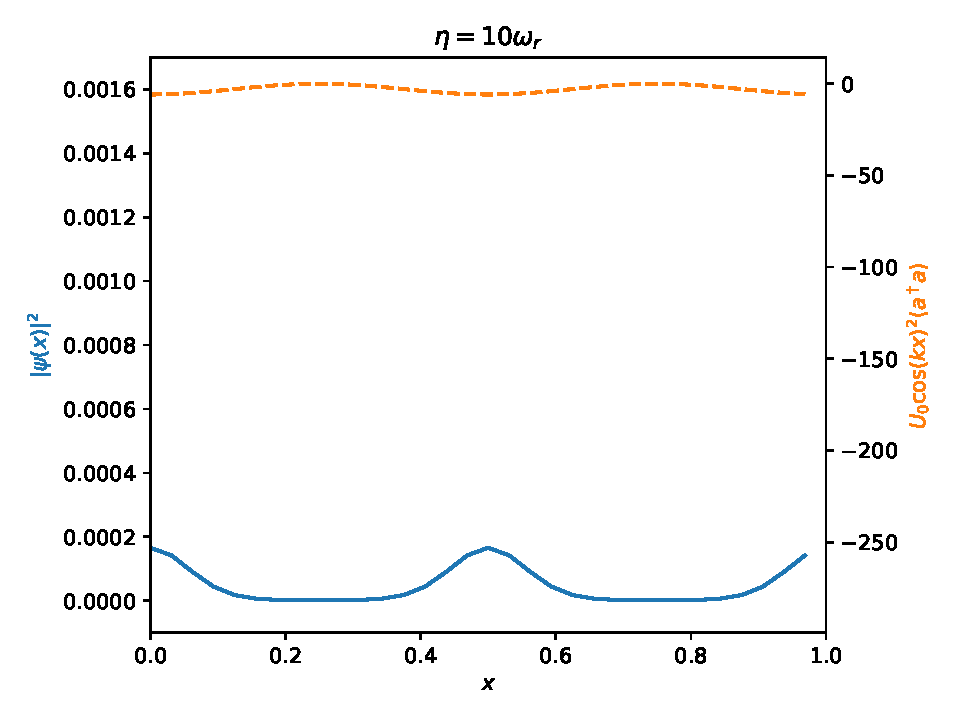
\includegraphics[width=.3\textwidth]{long_eta_10.pdf}\hfill
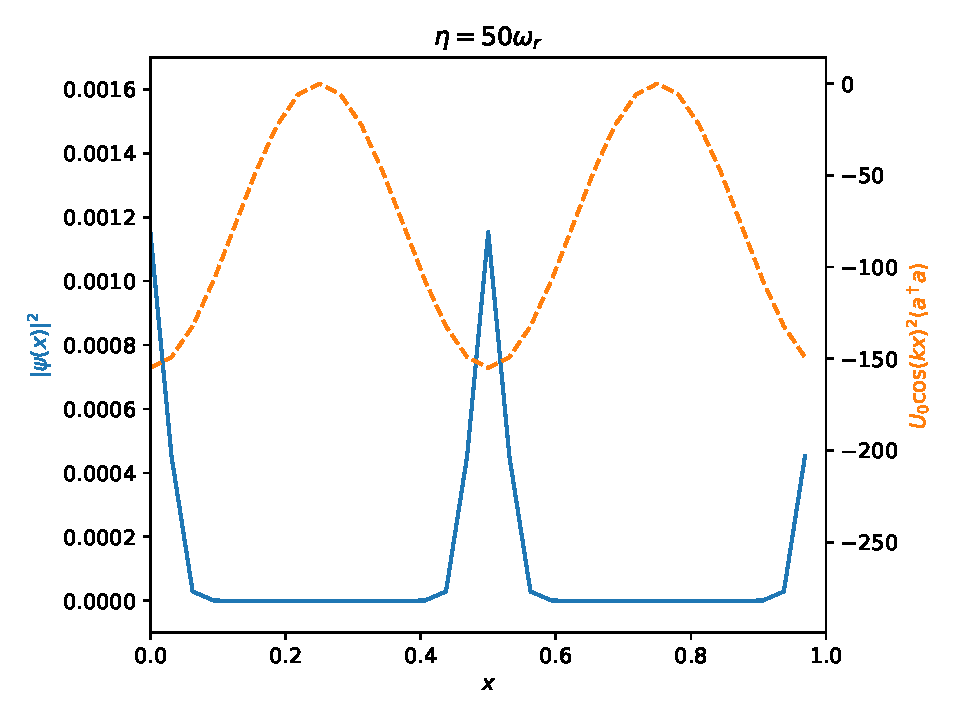
\includegraphics[width=.3\textwidth]{long_eta_50.pdf}\hfill
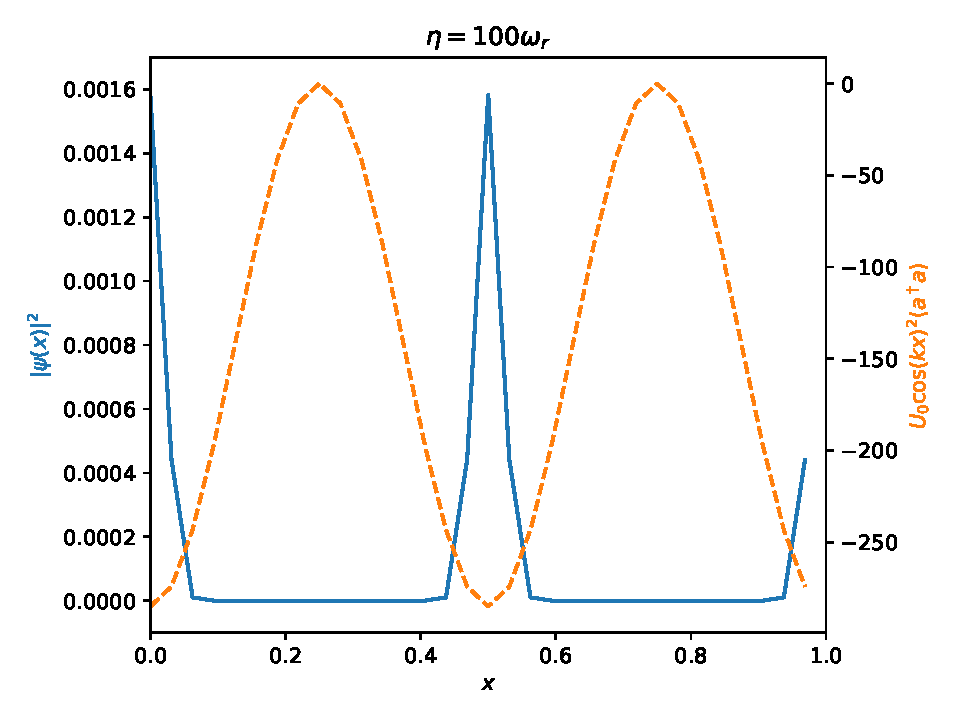
\includegraphics[width=.3\textwidth]{long_eta_100.pdf}
\caption{Longitudinal wave function densities for $\eta = 10 \omega_r$, $\eta = 50 \omega_r$ and $\eta = 100 \omega_r$.}
\label{long_eta}
\end{figure}
\FloatBarrier

\noindent Figures \ref{long_pmp_bunch} and \ref{trans_pmp_bunch} depict the bunching parameter $\langle \cos(kx)^2 \rangle$ each. We did not obtain any meaningful results with the order parameter $\langle \cos(kx) \rangle$.

\begin{figure}[ht]
  \centering
  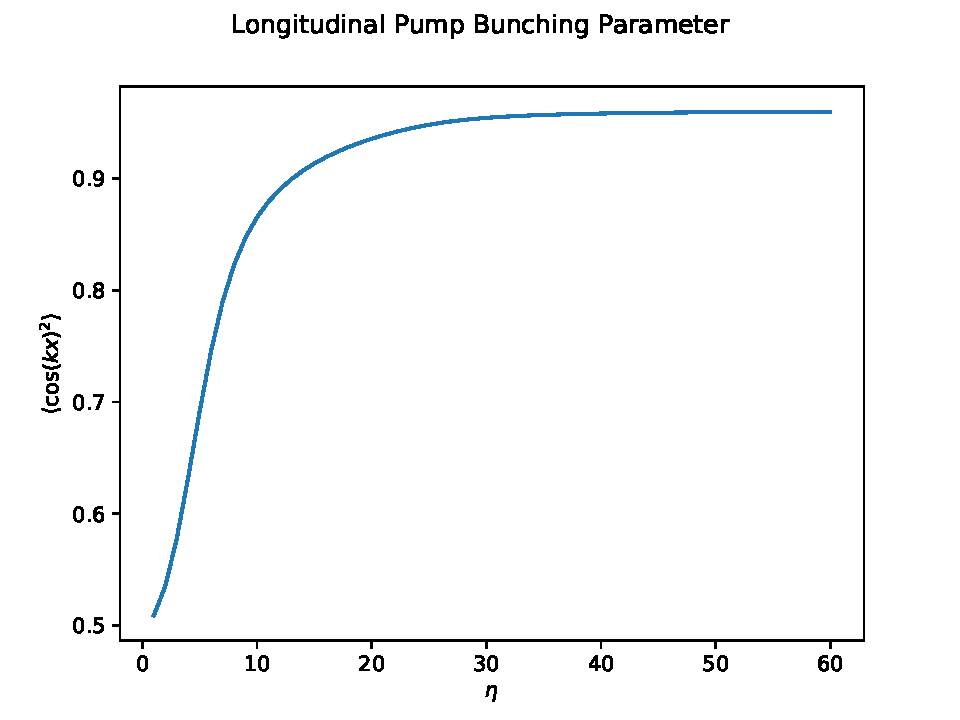
\includegraphics[width=.7\linewidth]{long_pmp_bunch.pdf}
  \caption{Bunching parameter for longitudinal pump with $\Delta_c = -10 \omega_r$ and $U_0 = -1 \omega_r$.}
  \label{long_pmp_bunch}
\end{figure}
\FloatBarrier

\begin{figure}[ht]
  \centering
  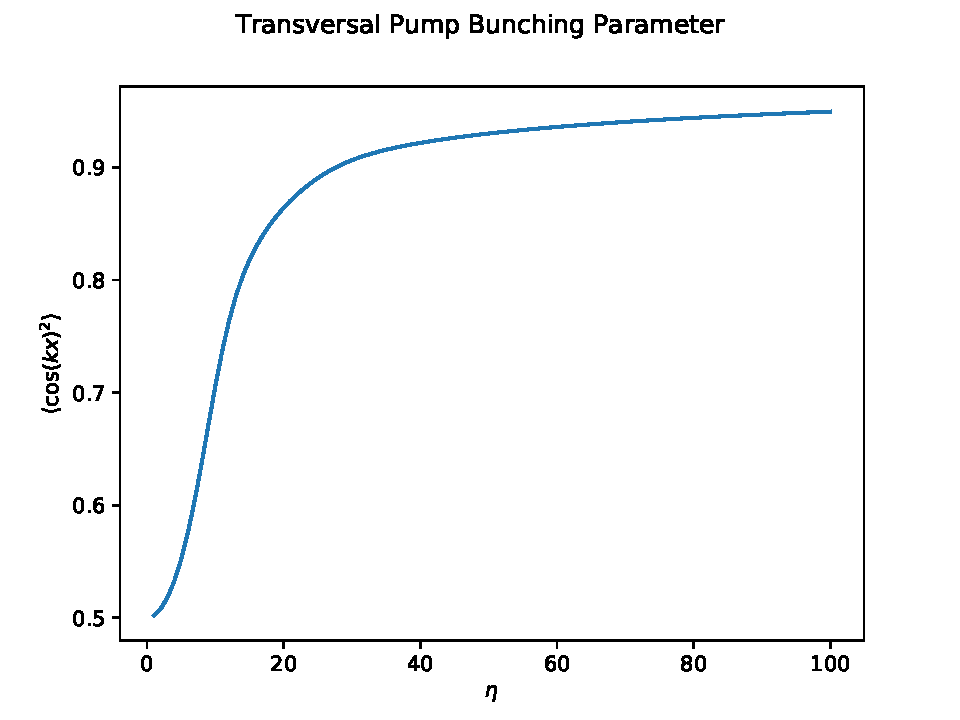
\includegraphics[width=.7\linewidth]{trans_pmp_bunch.pdf}
  \caption{Bunching parameter for transversal pump with $\Delta_c = -10 \omega_r$ and $U_0 = -1 \omega_r$.}
  \label{trans_pmp_bunch}
\end{figure}
\FloatBarrier

\noindent To obtain the order parameter as a function of $\eta$ for transversal pump, we used the mean-field approximation, as depicted in \cite{cold_atoms}. For now, a simple Euler algorithm will do. The results can be seen in Figure~\ref{trans_pmp_order}. Strangely, there is no threshold at which order sets in, but rather a gradual shift. We also tried to tweak the parameters similar to \cite{Nagy2008}, which unfortunately made the wave function all but disappear.

\begin{figure}[ht]
  \centering
  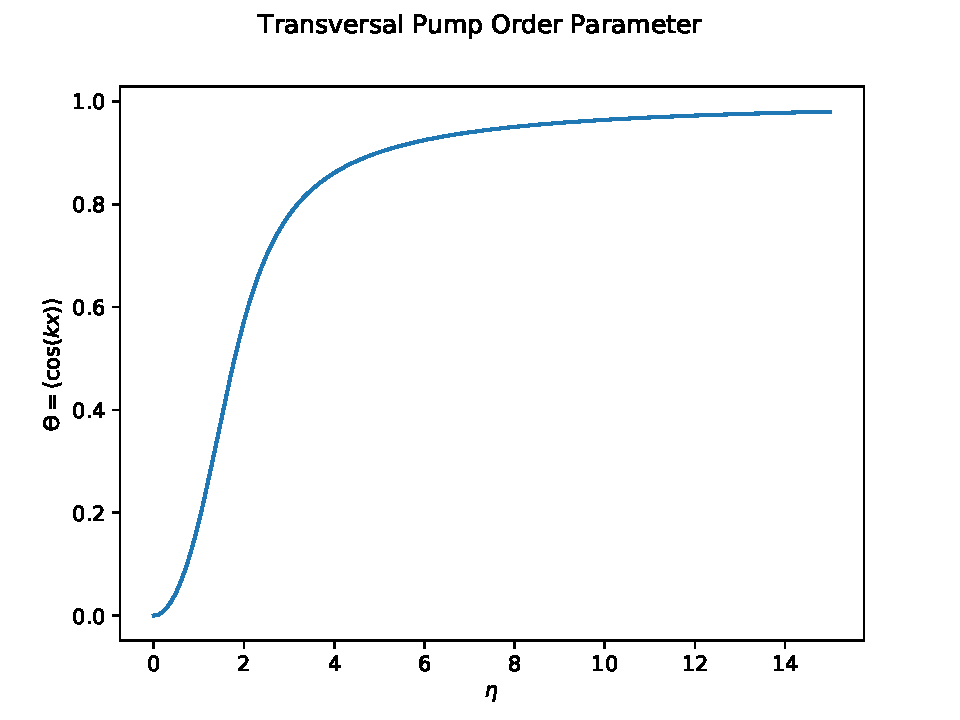
\includegraphics[width=.7\linewidth]{trans_pmp_order.pdf}
  \caption{Order parameter for transversal pump with $\Delta_c = -1 \omega_r$, $U_0 = -1 \omega_r$ and $\kappa = \omega_r$.}
  \label{trans_pmp_order}
\end{figure}
\FloatBarrier


\newpage

\bibliographystyle{unsrt}
\bibliography{bibliography}



\end{document}
